\documentclass{astroedu-lab}

\begin{document}

\pagestyle{plain}

\begin{problem}{\huge Лабораторная работа 1.2.5\\\\Исследование прецессии гироскопа\\\\Выполнил Жданов Елисей Б01-205}

\section{Цель работы:}

1) Исследовать вынужденную прецессию гироскопа

2) Установить зависимость скорости вынужденной прецессии от величины момента сил, действующих на ось гироскопа

3) Определить скорость вращения ротора гироскопа и сравнить её со скоростью, рассчитанной по скорости прецессии

\section{Оборудование:}

1) Гироскоп в кардановом подвесе

2) Секундомер

3) Набор грузов

4) Отдельный ротор гироскопа

5) Цилиндр известной массы

6) Крутитьный маятник

7) Штангенциркуль

8) Линейкка

\section{Теория гироскопа:}

Момент импульса твердого тела в его главных осях x, y, z равен

\begin{equation}
	\vec L = \vec i I_x \omega_x + \vec j I_y \omega_y + \vec k I_z \omega_z
\end{equation}

где $I_i$ - главные моменты инерции, $\omega_i$ - компоненты вектора угловой скорости.

Гироскопом же называется быстровращающееся тело, для которого момент импульса вдоль одной из осей много больше 2-х других.

\begin{wrapfigure}{r}{0.45\textwidth}
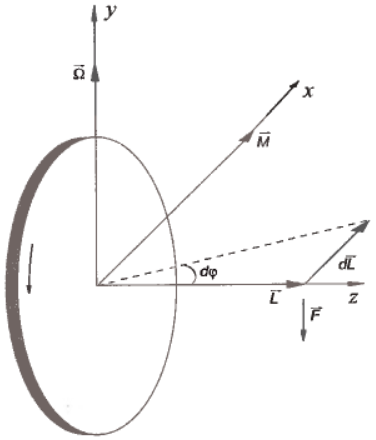
\includegraphics[width=0.45\textwidth]{theory_1.png}
\caption{}
\label{ris:image}
\end{wrapfigure}.

Выясним, какие силы надо приложить к гироскопу, чтобы изменить направление его оси. Рассмотрим для примера маховик, вращающийся вокруг оси z, перпендикулярной плоскости маховика, т.е. $\omega_z = \omega_0$

Пусть ось вращения повернулась в плоскости zx по направлению к оси x на бесконечно малый угол $d \phi$. Такой поворот означает добавочное вращение маховика вокруг оси y, так что

\begin{equation}
	d \phi = \Omega d t
\end{equation}

, где $\Omega$ - угловая скорость такого вращения. Будем предполагать, что

\begin{equation}
	L_{\Omega} \ll L_{\omega_0} \tag{1}
\end{equation}

Это значит, что изменением величины момента импульса маховика можно пренебречь, поскольку он всего-лишь повернется в плоскости zx. Таким образом

\begin{equation}
	|d \vec L| = L d \phi = L \Omega d t
\end{equation}

Поскольку это изменение направлено вдоль оси x, его удобно представить в виде векторного произведения

\begin{equation}
	|d \vec L| = \vec \Omega \times \vec L dt
\end{equation}

Тогда деля на dt

\begin{equation}
	\vec M = \vec \Omega \times \vec L
\end{equation}

Под действием момента внешних сил $\vec M$ ось гироскопа медленно вращается вокруг оси y с угловой скоростью $\Omega$. Такое движение называется регулярной прецессией гироскопа. В частности, создающей момент внешней силой может оказаться сила тяжести, если центр масс гироскопа не совпадает с точкой подвеса. Для гироскопа массой $m_{\text{г}}$, у которого ось собственного вращения наклонена на угол $\alpha$ от вертикали, скорость прецессии, происходящей вокруг вертикальной оси под действием силы тяжести, равна

\begin{equation}
	\Omega = \frac{M}{I_z \omega_0 \sin{\alpha}} = \frac{m_\text{г} g l_\text{ц}}{I_z \omega_0}
\end{equation}

$l_\text{ц}$ - расстояние от точки подвеса до центра масс гироскопа, т.е. скорость прецессии не зависит от $\alpha$.

Для изучения решулярной прецессии уравновешенного гироскопа к его оси подвешивают дополнительные грузы. Это смещает общий центр масс и создает момент сил тяжести, вызывающий прецессию. Скорость прецессии в этом случае равна

\begin{equation}
	\Omega = \frac{m g l}{I_z \omega_0}
\end{equation}

где m - масса груза, l - расстояние от центра карданова подвеса до точки крепления груза на оси гироскопа.

\newpage

\section{Описание установки:}

\begin{wrapfigure}{r}{0.45\textwidth}
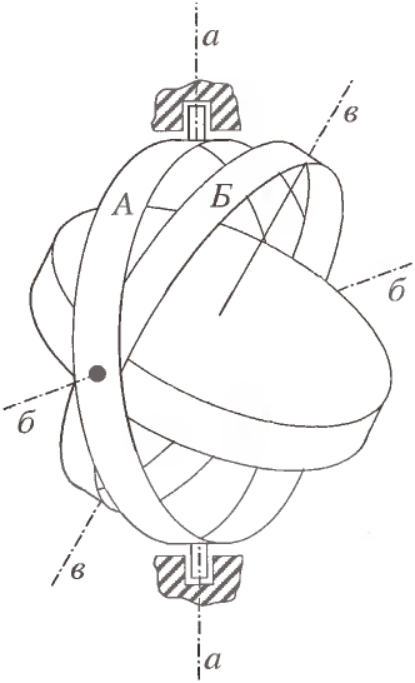
\includegraphics[width=0.45\textwidth]{state_1.png}
\caption{}
\label{ris:image}
\end{wrapfigure}.

В данной работе исследуется регулярная прецессия уравновешенного гироскопа.

Уравновешенный гироскоп, закрепленный в кольцах карданова подвеса, показан на рис. 2. Наружное кольцо подвеса A может свободно поворачиваться вокруг вертикальной оси aa. Внутреннее кольцо Б связано с кольцом А горизонтальной осью бб. В кольце Б закреплен гироскоп, ось вращения которого вв перпендикулярна оси бб. Центр масс гироскопа находится на пересечении всех трех осей и при любом повороте колец сохраняет свое положение в пространстве. Получается, что гироскоп как-бы подвешен за центр масс.

Экспериментальная установка для исследования прецессии гироскопа показана на рис.3. Ротором гироскопа является ротор высокооборотного электромотора M, питающегося током частотой 400 Гц. Статор скреплен с кольцом Б. Мотор с кольцом Б может вращаться в кольце А вокруг горизонтальной оси бб, которое может вращаться вокруг вертикальной оси аа. Ротор электромотора представляет собой массивный стальной цилиндр с прожилками меди, образующими беличье колесо. Обозначенный на рис. 3. буквой С рычаг направлен по оси симметрии ротора. На рычаг подвешивают грузы Г. Подвешивая различные грузы, можно менять силу F, момент которой определяется расстоянием l от точки подвеса до горизонтальной оси кольца A(до центра масс гироскопа), укказанным на самой установке.

\newpage

\begin{wrapfigure}{r}{0.45\textwidth}
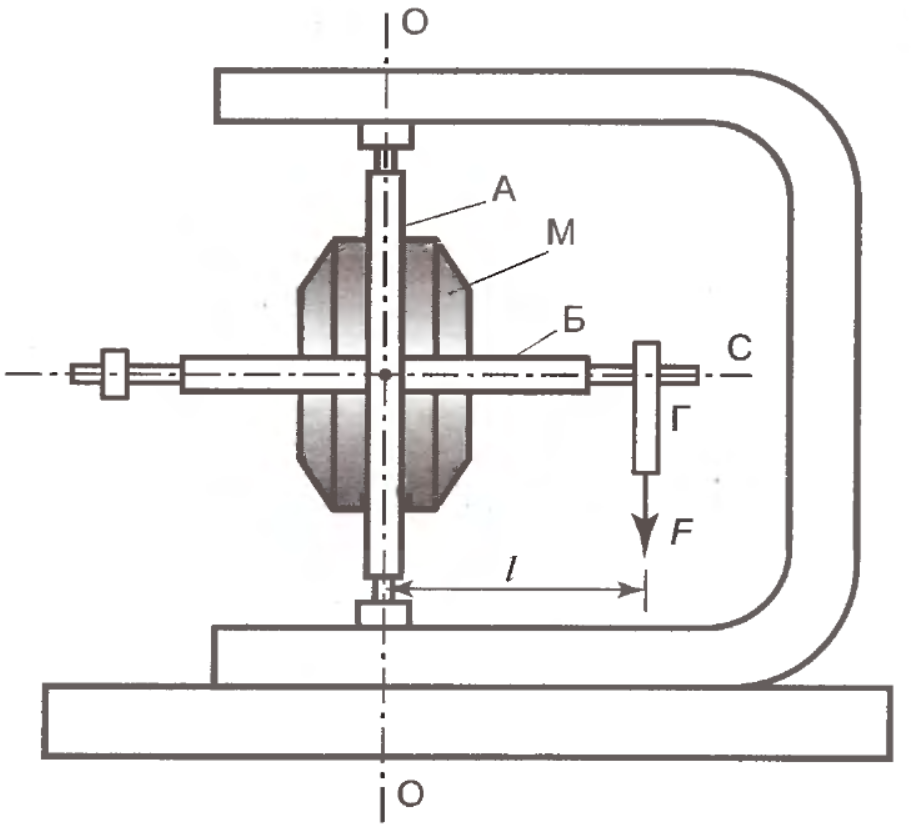
\includegraphics[width=0.45\textwidth]{state_2.png}
\caption{}
\label{ris:image}
\end{wrapfigure}.

Выше при выводе формул для прецессии предполагалось, что действующие на гироскоп сила лежат в плоскости zy, в которой лежат вектора угловых скоростей собственного вращения и прецессии. В этом случае момент сил меняет лишь направление момента импульса гироскопа, но не его величину. Силы трения не лежат в плоскоси осей вразения. Они приводят к изменению моментра импульса и по направлению, и по величине. Для ротора гироскопа действие сил трения скомпенсировано действием электромотора. Для осей карданова подвеса компенсации нет. В результате ось гироскопа будет опускаться в направлении действия груза.

Изменение скорости прецесии гироскопа позволяет вычислить угловую скорость вращения его ротора. Момент инерции ротора относительно оси симметрии $I_0$ измеряется по крутильным колебаниям точной комии ротора, подвешиваемой вдоль оси симметрии на жесткой проволке. Период крутильных колебаний $T_0$ определяется

\begin{equation}
	T_0 = 2 \pi \sqrt{\frac{I_0}{f}}
\end{equation}

Чтобы исключить модуль кручения проволки, вместо ротора гироскопа к той же проволке подвешивают цилиндр правильной формы с известными размерами и массой, для которого легко можно вычислить момент инерции $I_{\text{ц}}$. Для определения момента инерции ротора гироскопа имеем

\begin{equation}
	I_0 = I_\text{ц}\frac{T_0^2}{T_\text{ц}^2}
\end{equation}

Скорость вращения ротора гироскопа можно определить и не прибегая к исследованию прецессии. У используемых в работе гироскопов статор имеет две обмотки, необходимые для быстрой раскрутки гироскопа. В данной работе одну из обмоток используют для раскрутки гироскопа, а вторую - для измерения частоты оборотов ротора. Ротор всегда немного намагничен. Вращаясь, он наводит во второй обмотке переменную ЭДС индукции, частота которой равна частоте вращения ротора. Частоту этой ЭДС можно, в частности, измерить по фигурам Лиссажу, получаемым на экране осциллографа, если на один вход подать исследуемую ЭДС, а на другой - переменное напряжение с генератора. При совпадении частот на экране получаем эллипс.

\section{Измерения и обработка:}

1 - 2) Подключим гироскоп к питанию, заранее установив его в требуемое положение, пока он не раскрутился и это не стало затруднительно.

3) При воздействии силы вниз на горизонтальную ось гироскопа она движется против часовой стрелки. Вектор угловой скорости направлен вверх, момента силы - направо. Значит момент импульса и вектор угловой скорости гироскопа направлен вдоль оси в сторону точки приложения силы. Значит для такой оси вращение происходит против часовой стрелки.

4) Трение в оси карданова подвеса(а) позволит грузу вместе с осью опускаться вниз.

5 - 6) Запишу результаты замеров в таблицу

\begin{center}
\begin{tabular}[t]{|c|l|l|l|l|l|l|}
\hline
$m_i$, г & n & \multicolumn{3}{|c|}{t, с} & M, Н$\cdot$м & $\Omega$, с$^{-1}$ \\
\hline
&& $t_1$ & $t_2$ & $\overline{t}$ && \\
\hline
343 & 6 & 178.84 & 177.94 & 178.39 & 0.400 & 0.211 \\
267 & 5 & 189.83 & 190.94 & 190.39 & 0.312 & 0.165 \\
215 & 4 & 193.16 & 199.19 & 196.18 & 0.251 & 0.128 \\
141 & 3 & 216.00 & 216.41 & 216.21 & 0.165 & 0.087 \\
112 & 3 & 274.06 & 274.03 & 274.05 & 0.131 & 0.069 \\
93  & 3 & 326.44 & 326.44 & 326.44 & 0.109 & 0.058 \\
76  & 2 & 270.84 & 273.31 & 272.08 & 0.089 & 0.046 \\
\hline
\end{tabular}
\end{center} 

$m_i$ - масса очередного груза, n - количество полных оборотов, t - соответствующее им время.

Было принято решение делать 2 замера, поскольку целое количество оборотов для груза всегда совпадало, а время отличалось с точностью до реакции экспериментатора, при этом сильно большую погрешность вносит именно метод замера по целым оборотам.

Усредненный момент силы составит

\begin{equation}
	M = m g l
\end{equation}

Длина l составляет 119 мм(указано на установке).

Ускорение свободного падения возьму $g = 9.815$ м/c$^2$.

\begin{center}
\begin{tikzpicture}
\begin{axis}[
	width=250,
	xlabel     = \text{$M$ [Н $\cdot$ м]$^2$}, % label x axis
    ylabel     = \text{$\Omega$ [с]$^-1$}, % label y axis
	]
\addplot[mark = *, only marks] table {
	x     y
0.089 0.046
0.109 0.058
0.131 0.069
0.165 0.087
0.251 0.128
0.312 0.165
0.400 0.211
};

\addplot[mark = ] table {
	x     y
0 -0.00047
0.4 0.210
};
\end{axis}
\end{tikzpicture}
\end{center}

Коэффициент наклона

\begin{equation}
	k = \frac{1}{I_z \omega_0} = 0.527 \pm 0.005 \text{ [СИ]}
\end{equation}

7 - 8) Масса пробника - 1.6169 кг, его радиус вычисляется из замера диаметра штангенциркулем и составляет 3.9 см.

Период колебаний пробника найду из длительности 10 подряд идущих колебаний. $T_\text{ц} = \frac{40.41}{10} = 4.04 \pm 0.02$ сек.

Период колебаний ротора $T_\text{0} = \frac{64.09}{20} = 3.20 \pm 0.01$

Тогда искомый момент инерции

\begin{equation}
	I_0 = \frac{1}{2} m r^2 \cdot \frac{T_0^2}{T_\text{ц}^2} = (7.71 \pm 0.17) \cdot 10^{-4} \text{ кг} \cdot \text{м}^2
\end{equation}

9) Наконец частота вращения гироскопа вокруг оси z

\begin{equation}
	\boxed{\omega_0 = \frac{1}{I_z k} = (2460 \pm 80) \text{ c}^{-1}}
\end{equation}

10) Скорость опускания рычага для выбранных углов($6^\circ$ и полный оборот) связана со скоростью вращения

\begin{equation}
	\Delta \Omega_{\text{уд}} = \frac{12^\circ}{360^\circ} \Omega_{\text{уд}} = 0.0205 \text{ с}^{-1}
\end{equation}

Итого момент сил трения

\begin{equation}
	\boxed{m_{\mu} = m_{g} \frac{12^\circ}{360^\circ} = 0.039 \text{ м}^2 / \text{с}^2}
\end{equation}

Выражение просто следует из разложения движения гироскопа по двум осям. Вдоль каждого направления движение связано с соответствующим моментом сил. Пропорциональным моментам сил будет соответствовать пропорциональная скорость прецессии.

Был произведен расчет для удельной массы(на килограммовый груз)

11) Приведу полученную таблицу с замерами и соответствующий график.
\begin{center}
\begin{tabular}[t]{|l|l|}
\hline
$\tau$, сек & $\nu$, Гц \\
\hline
15  & 385.6 \\
30  & 381.3 \\
38  & 378.3 \\
49.5& 375.6 \\
65  & 371.3 \\
80  & 366.5 \\
100 & 361.4 \\
120 & 356.1 \\
140 & 351.0 \\
160 & 345.5 \\
180 & 339.9 \\
200 & 335.1 \\
220 & 333.5 \\

\hline
\end{tabular}
\end{center}

\begin{center}
\begin{tikzpicture}
\begin{axis}[
	width=250,
	xlabel     = \text{$\tau$, сек}, % label x axis
    ylabel     = \text{$\nu$, Гц}, % label y axis
	]
\addplot[mark = *, only marks] table {
	x     y
15   385.6
30   381.3
38   378.3
49.5 375.6
65   371.3
80   366.5
100  361.4
120  356.1
140  351.0
160  345.5
180  339.9
200  335.1
220  333.5
};

\addplot[mark = ] table {
	x     y
0 389.2
220 328.7 
};
\end{axis}
\end{tikzpicture}
\end{center}

В итоге

\begin{equation}
	\nu_0 = 389.2 \text{ Гц}
\end{equation}

\begin{equation}
	\boxed{\omega_0 = 2 \pi \nu_0 = (2445.4 \pm 0.6) \text{ с}^{-1}}
\end{equation}

Замечу, что вследствии того, что гироскопу необходимо действительно(бесконечно) большое время, чтобы досчить своей максимальной частоты вращения, реальная погрешность может быть большей.

\section{Время делать выводы:}

12 - 13, п3 цели) Частоты, замеренные 2-мя различными способами, отличаются буквально на процент, что я считаю отличным результатом. Поэтому формула (5)(книжный индекс) действительно применима с имеющимися приближениями. Более того, принятые теоретические приближения как обычно не сыграли роли в погрешности, поскольку были более веские практические факторы эксперимента, которые не позволяли сравнять приборную и теоретическую погрешности.

Поэтому считаю, что вынужденная прецессия гироскопа исследована исчерпывающе различными способами и цель работы выполнена.

\end{problem}
\end{document}